% Figure 17 -- 3d mirrors for the AD theories of Examples 1, 2, 3
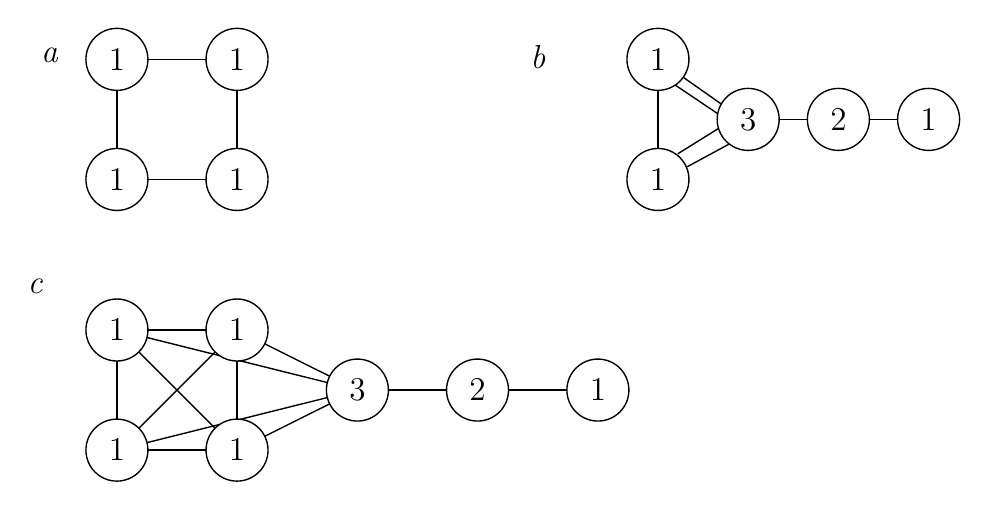
\begin{tikzpicture}[x=1pt,y=1pt,>=stealth,line width=0.5pt,
   nd/.style={circle,draw,fill=white,minimum size=22.4pt,inner sep=0pt}]
  % ===================== a) =====================
  \draw (37.6,164.0) rectangle (81.0,120.6);
  % ===================== b) =====================
  \draw (233.1,164.0) -- (233.1,120.6);
  \draw (238.3,155.4) -- (255.1,144.1);
  \draw (242.4,157.4) -- (256.5,147.5);
  \draw (240.3,129.9) -- (255.1,139.1);
  \draw (243.7,125.2) -- (259.2,133.6);
  \draw (265.7,142.3) -- (298.3,142.3) -- (330.9,142.3);
  % ===================== c) =====================
  \draw (37.6,66.2) -- (81.0,66.2) -- (81.0,22.8) -- (37.6,22.8) -- cycle;
  \draw (37.6,66.2) -- (81.0,22.8);
  \draw (37.6,22.8) -- (81.0,66.2);
  \draw (37.6,66.2) -- (124.5,44.5);
  \draw (81.0,66.2) -- (124.5,44.5);
  \draw (37.6,22.8) -- (124.5,44.5);
  \draw (81.0,22.8) -- (124.5,44.5);
  \draw (124.5,44.5) -- (167.9,44.5) -- (211.4,44.5);
  % ===================== nodes =====================
  \foreach \x/\y in {37.6/164.0,81.0/164.0,81.0/120.6,37.6/120.6}
    {\node[nd] at (\x,\y) {\fontsize{12}{14}\selectfont 1};}
  \foreach \x/\y in {233.1/164.0,233.1/120.6}
    {\node[nd] at (\x,\y) {\fontsize{12}{14}\selectfont 1};}
  \node[nd] at (265.7,142.3) {\fontsize{12}{14}\selectfont 3};
  \node[nd] at (298.3,142.3) {\fontsize{12}{14}\selectfont 2};
  \node[nd] at (330.9,142.3) {\fontsize{12}{14}\selectfont 1};
  \foreach \x/\y in {37.6/66.2,81.0/66.2,37.6/22.8,81.0/22.8}
    {\node[nd] at (\x,\y) {\fontsize{12}{14}\selectfont 1};}
  \node[nd] at (124.5,44.5) {\fontsize{12}{14}\selectfont 3};
  \node[nd] at (167.9,44.5) {\fontsize{12}{14}\selectfont 2};
  \node[nd] at (211.4,44.5) {\fontsize{12}{14}\selectfont 1};
  % ===================== panel letters =====================
  \node[inner sep=0pt] at (13.1,165.45) {\fontsize{12}{14}\itshape a};
  \node[inner sep=0pt] at (189.7,164.75) {\fontsize{12}{14}\itshape b};
  \node[inner sep=0pt] at (8.05,81.9)   {\fontsize{12}{14}\itshape c};
\end{tikzpicture}
